\documentclass[11pt,a4paper]{article}
%%%%%%%%%%%%%%%%%%%%%%%%% Credit %%%%%%%%%%%%%%%%%%%%%%%%

% template ini dibuat oleh martin.manullang@if.itera.ac.id untuk dipergunakan oleh seluruh sivitas akademik itera.

%%%%%%%%%%%%%%%%%%%%%%%%% PACKAGE starts HERE %%%%%%%%%%%%%%%%%%%%%%%%
\usepackage{graphicx}
\usepackage{caption}
\usepackage{microtype}
\usepackage{multicol}
\usepackage{lmodern}
\captionsetup[table]{name=Tabel}
\captionsetup[figure]{name=Gambar}
\usepackage{tabulary}
\usepackage{minted}
\usepackage{amsmath}
\usepackage{fancyhdr}
\usepackage{amssymb}
\usepackage{amsthm}
\usepackage{placeins}
\usepackage{amsfonts}
\usepackage{graphicx}
\usepackage[all]{xy}
\usepackage{tikz}
\usepackage{verbatim}
\usepackage[left=2cm,right=2cm,top=3cm,bottom=2.5cm]{geometry}
\usepackage{hyperref}
\hypersetup{
    colorlinks,
    linkcolor={red!50!black},
    citecolor={blue!50!black},
    urlcolor={blue!80!black}
}
\usepackage{caption}
\usepackage{subcaption}
\usepackage{multirow}
\usepackage{psfrag}
\usepackage[T1]{fontenc}
\usepackage[scaled]{beramono}
% Enable inserting code into the document
\usepackage{listings}
\usepackage{xcolor} 
% custom color & style for listing
\definecolor{codegreen}{rgb}{0,0.6,0}
\definecolor{codegray}{rgb}{0.5,0.5,0.5}
\definecolor{codepurple}{rgb}{0.58,0,0.82}
\definecolor{backcolour}{rgb}{0.95,0.95,0.92}
\definecolor{LightGray}{gray}{0.9}
\lstdefinestyle{mystyle}{
	backgroundcolor=\color{backcolour},   
	commentstyle=\color{green},
	keywordstyle=\color{codegreen},
	numberstyle=\tiny\color{codegray},
	stringstyle=\color{codepurple},
	basicstyle=\ttfamily\footnotesize,
	breakatwhitespace=false,         
	breaklines=true,                 
	captionpos=b,                    
	keepspaces=true,                 
	numbers=left,                    
	numbersep=5pt,                  
	showspaces=false,                
	showstringspaces=false,
	showtabs=false,                  
	tabsize=2
}
\lstset{style=mystyle}
\renewcommand{\lstlistingname}{Kode}
%%%%%%%%%%%%%%%%%%%%%%%%% PACKAGE ends HERE %%%%%%%%%%%%%%%%%%%%%%%%


%%%%%%%%%%%%%%%%%%%%%%%%% Data Diri %%%%%%%%%%%%%%%%%%%%%%%%
\newcommand{\student}{\textbf{Rizki Alfariz Ramadhan (122140061)}}
\newcommand{\course}{\textbf{Sistem Teknologi Multimedia (IF25-40305)}}
\newcommand{\assignment}{\textbf{Worksheet 1: Setup Python Environment untuk Multimedia}}

%%%%%%%%%%%%%%%%%%% using theorem style %%%%%%%%%%%%%%%%%%%%
\newtheorem{thm}{Theorem}
\newtheorem{lem}[thm]{Lemma}
\newtheorem{defn}[thm]{Definition}
\newtheorem{exa}[thm]{Example}
\newtheorem{rem}[thm]{Remark}
\newtheorem{coro}[thm]{Corollary}
\newtheorem{quest}{Question}[section]
%%%%%%%%%%%%%%%%%%%%%%%%%%%%%%%%%%%%%%%%
\usepackage{lipsum}%% a garbage package you don't need except to create examples.
\usepackage{fancyhdr}
\pagestyle{fancy}
\lhead{Rizki Alfariz Ramadhan (122140061)}
\rhead{ \thepage}
\cfoot{\textbf{Worksheet 1: Setup Python Environment untuk Multimedia}}
\renewcommand{\headrulewidth}{0.4pt}
\renewcommand{\footrulewidth}{0.4pt}

%%%%%%%%%%%%%%  Shortcut for usual set of numbers  %%%%%%%%%%%

\newcommand{\N}{\mathbb{N}}
\newcommand{\Z}{\mathbb{Z}}
\newcommand{\Q}{\mathbb{Q}}
\newcommand{\R}{\mathbb{R}}
\newcommand{\C}{\mathbb{C}}
\setlength\headheight{14pt}

%%%%%%%%%%%%%%%%%%%%%%%%%%%%%%%%%%%%%%%%%%%%%%%%%%%%%%%555
\begin{document}
\thispagestyle{empty}
\begin{center}
	
\includegraphics[scale = 0.15]{Figure/ifitera-header.png}
	\vspace{0.1cm}
\end{center}
\noindent
\rule{17cm}{0.2cm}\\[0.3cm]
Nama: \student \hfill Tugas Ke: \assignment\\[0.1cm]
Mata Kuliah: \course \hfill Tanggal: \today\\
\rule{17cm}{0.05cm}
\vspace{0.1cm}



%%%%%%%%%%%%%%%%%%%%%%%%%%%%%%%%%%%%%%%%%%%%% BODY DOCUMENT %%%%%%%%%%%%%%%%%%%%%%%%%%%%%%%%%%%%%%%%%%%%%
\section{Instruksi Tugas}

\subsection{Persiapan}
\textbf{Sebelum memulai, pastikan Anda telah:}
\begin{itemize}
    \item Menginstall Python 3.8 atau lebih baru di sistem Anda. Versi python yang digunakan adalah 3.10.18
    \item Memilih salah satu tool manajemen environment: \textbf{conda}, \textbf{venv}, atau \textbf{uv}. Salah satu tool manjemen environment yang digunakan adalah \textbf{uv}.
    \item Membuka terminal/command prompt
    \item Menyiapkan dokumen \LaTeX\ ini untuk dokumentasi
\end{itemize}

\subsection{Bagian 1: Membuat Environment Python}

\subsubsection{Opsi 3: Menggunakan uv (Modern dan cepat)}
\begin{lstlisting}[language=bash, caption=Membuat environment dengan uv]
# Install uv terlebih dahulu jika belum ada
pip install uv

# Jika menggunakan PowerShell (Windows)
powershell -ExecutionPolicy ByPass -c "irm https://astral.sh/uv/install.ps1 | iex"

# Membuat environment baru
uv venv multimedia-uv

# Mengaktifkan environment (Windows)
multimedia-uv\Scripts\activate

# Downgrade versi Python
uv python install 3.10

# Verifikasi environment aktif (Windows PowerShell)
Get-Command python
\end{lstlisting}

\textbf{Dokumentasikan di sini:}
\begin{itemize}
    \item Tool manajemen environment yang Anda pilih: \textbf{[UV]}
    \item Screenshot atau copy-paste output dari perintah verifikasi environment
    \begin{figure}[h!]
    \centering
    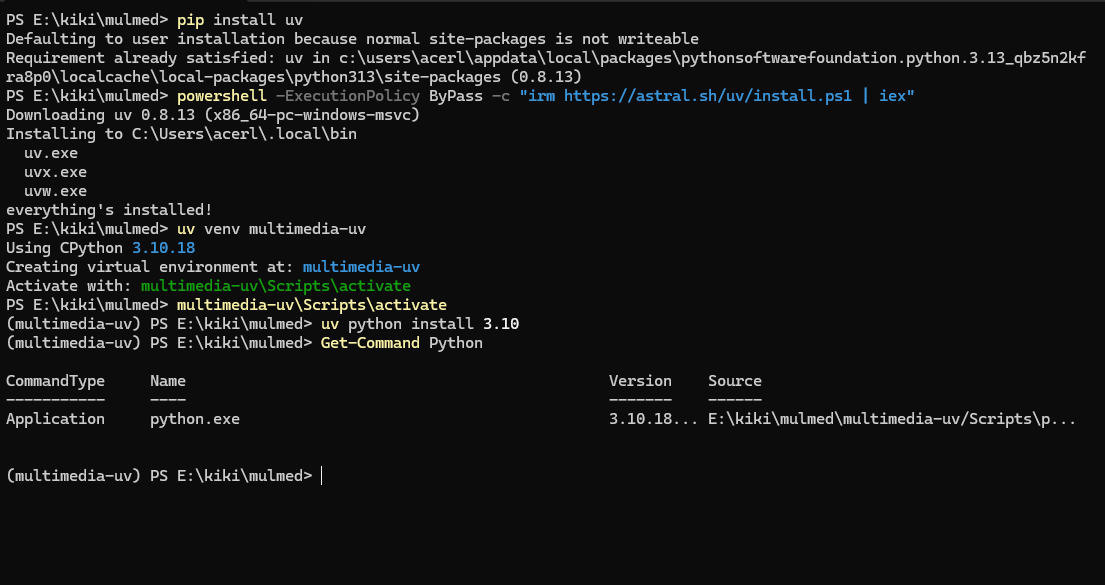
\includegraphics[scale = 0.5]{Figure/Install-UV1.png}
    \caption{Output perintah verifikasi environment}
    \vspace{0.1cm}
    \end{figure}
\end{itemize}

\subsection{Bagian 2: Instalasi Library Multimedia}
Setelah environment aktif, install library-library berikut:

\subsubsection{Library Audio Processing}
\begin{lstlisting}[language=bash, caption=Instalasi library audio]
# Untuk pip (venv/uv):
pip install librosa soundfile scipy
\end{lstlisting}

\subsubsection{Library Image Processing}
\begin{lstlisting}[language=bash, caption=Instalasi library image]
# Untuk pip (venv/uv):
pip install opencv-python pillow scikit-image matplotlib
\end{lstlisting}

\subsubsection{Library Video Processing}
\begin{lstlisting}[language=bash, caption=Instalasi library video]
# Untuk pip (venv/uv):
pip install moviepy ffmpeg
\end{lstlisting}

\subsubsection{Library General Purpose}
\begin{lstlisting}[language=bash, caption=Instalasi library umum]
# Untuk pip (venv/uv):
pip install numpy pandas jupyter
\end{lstlisting}

\textbf{Dokumentasikan di sini:}
\begin{itemize}
    \item Perintah instalasi yang Anda gunakan:
        \begin{itemize}
            \item Audio : \texttt{uv pip install librosa soundfile scipy}
            \item Image: \texttt{uv pip install opencv-python pillow scikit-image matplotlib}
            \item Video: \texttt{uv pip install moviepy ffmpeg}
            \item General: \texttt{uv pip install numpy pandas jupyter}
        \end{itemize}
    \item Screenshot proses instalasi atau output sukses
        \begin{figure}[h]
            \centering
            \begin{subfigure}{0.48\textwidth}
                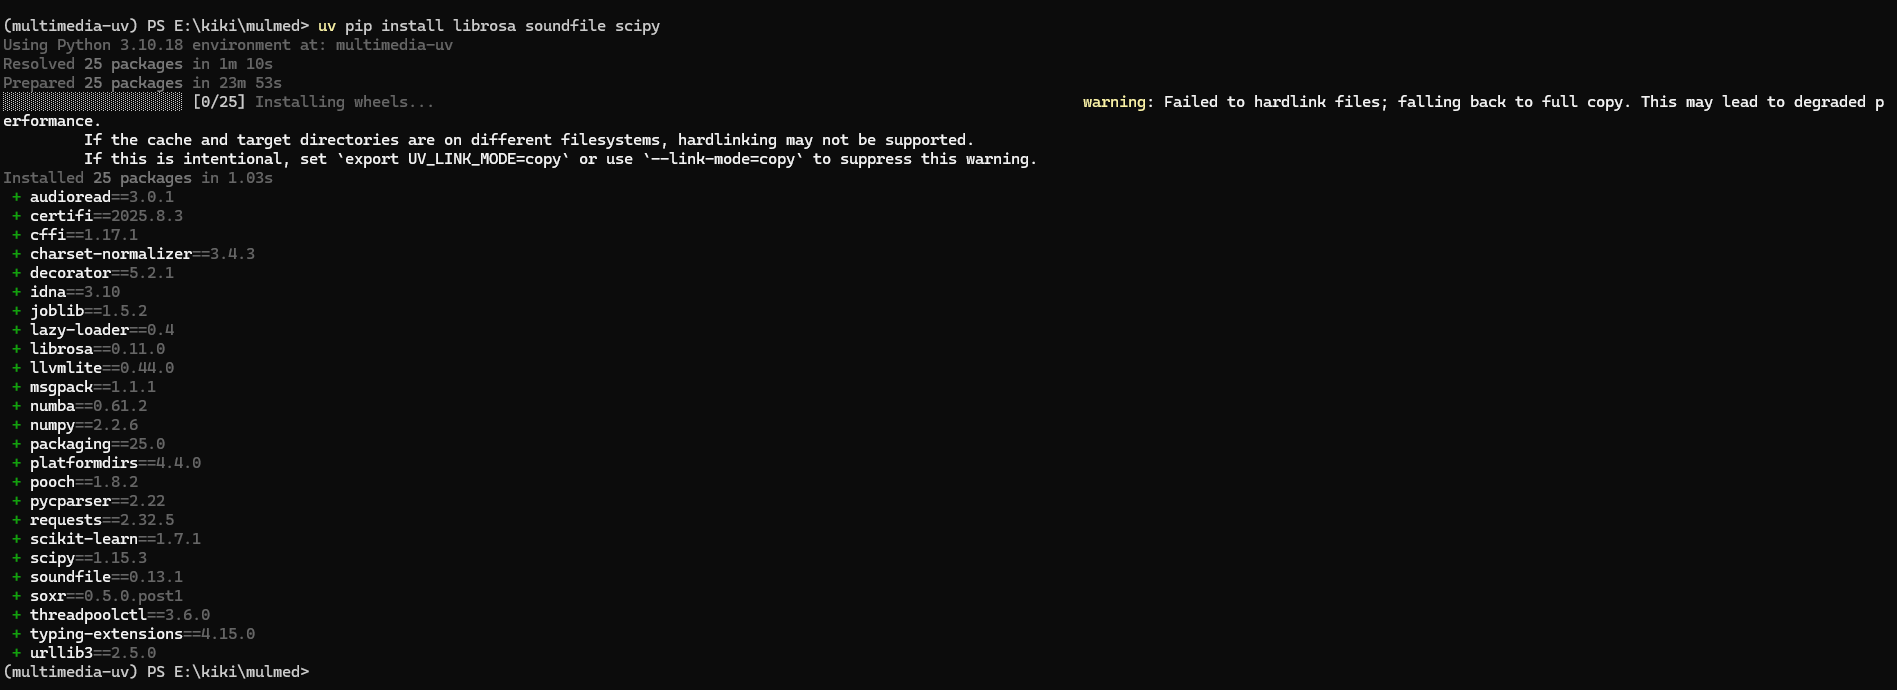
\includegraphics[width=\linewidth]{Figure/InstallAudio.png}
                \caption{Instalasi library audio processing}
            \end{subfigure}
            \begin{subfigure}{0.48\textwidth}
                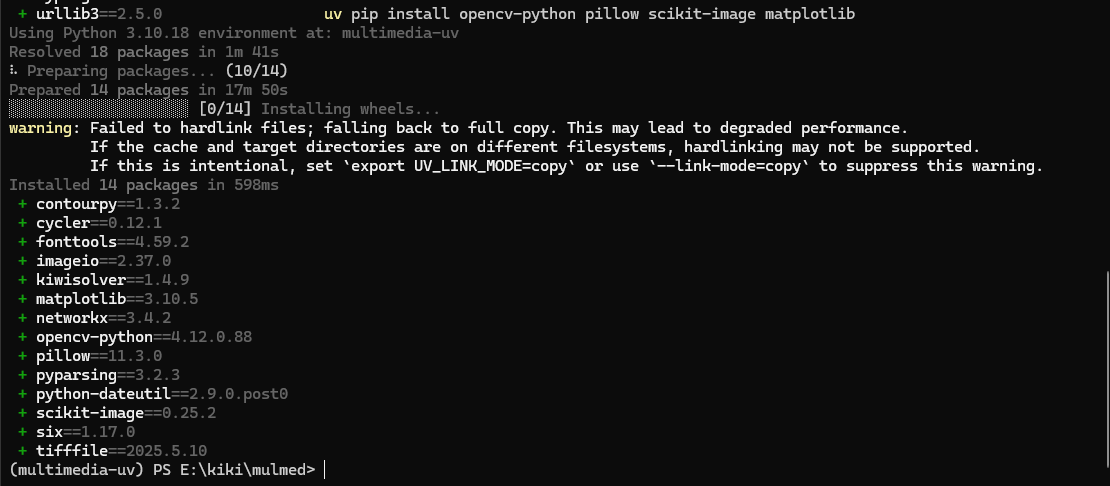
\includegraphics[width=\linewidth]{Figure/InstallImage.png}
                \caption{Instalasi library image processing}
            \end{subfigure}
            \begin{subfigure}{0.48\textwidth}
                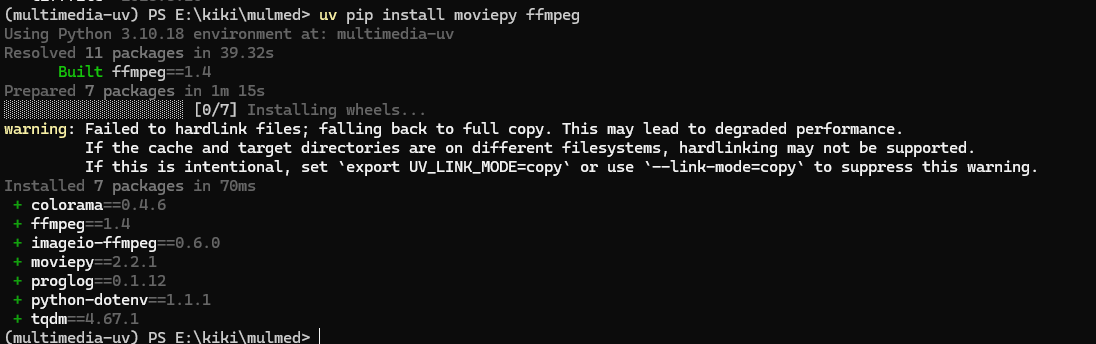
\includegraphics[width=\linewidth]{Figure/InstallVideo.png}
                \caption{Instalasi library video processing}
            \end{subfigure}
            \begin{subfigure}{0.48\textwidth}
                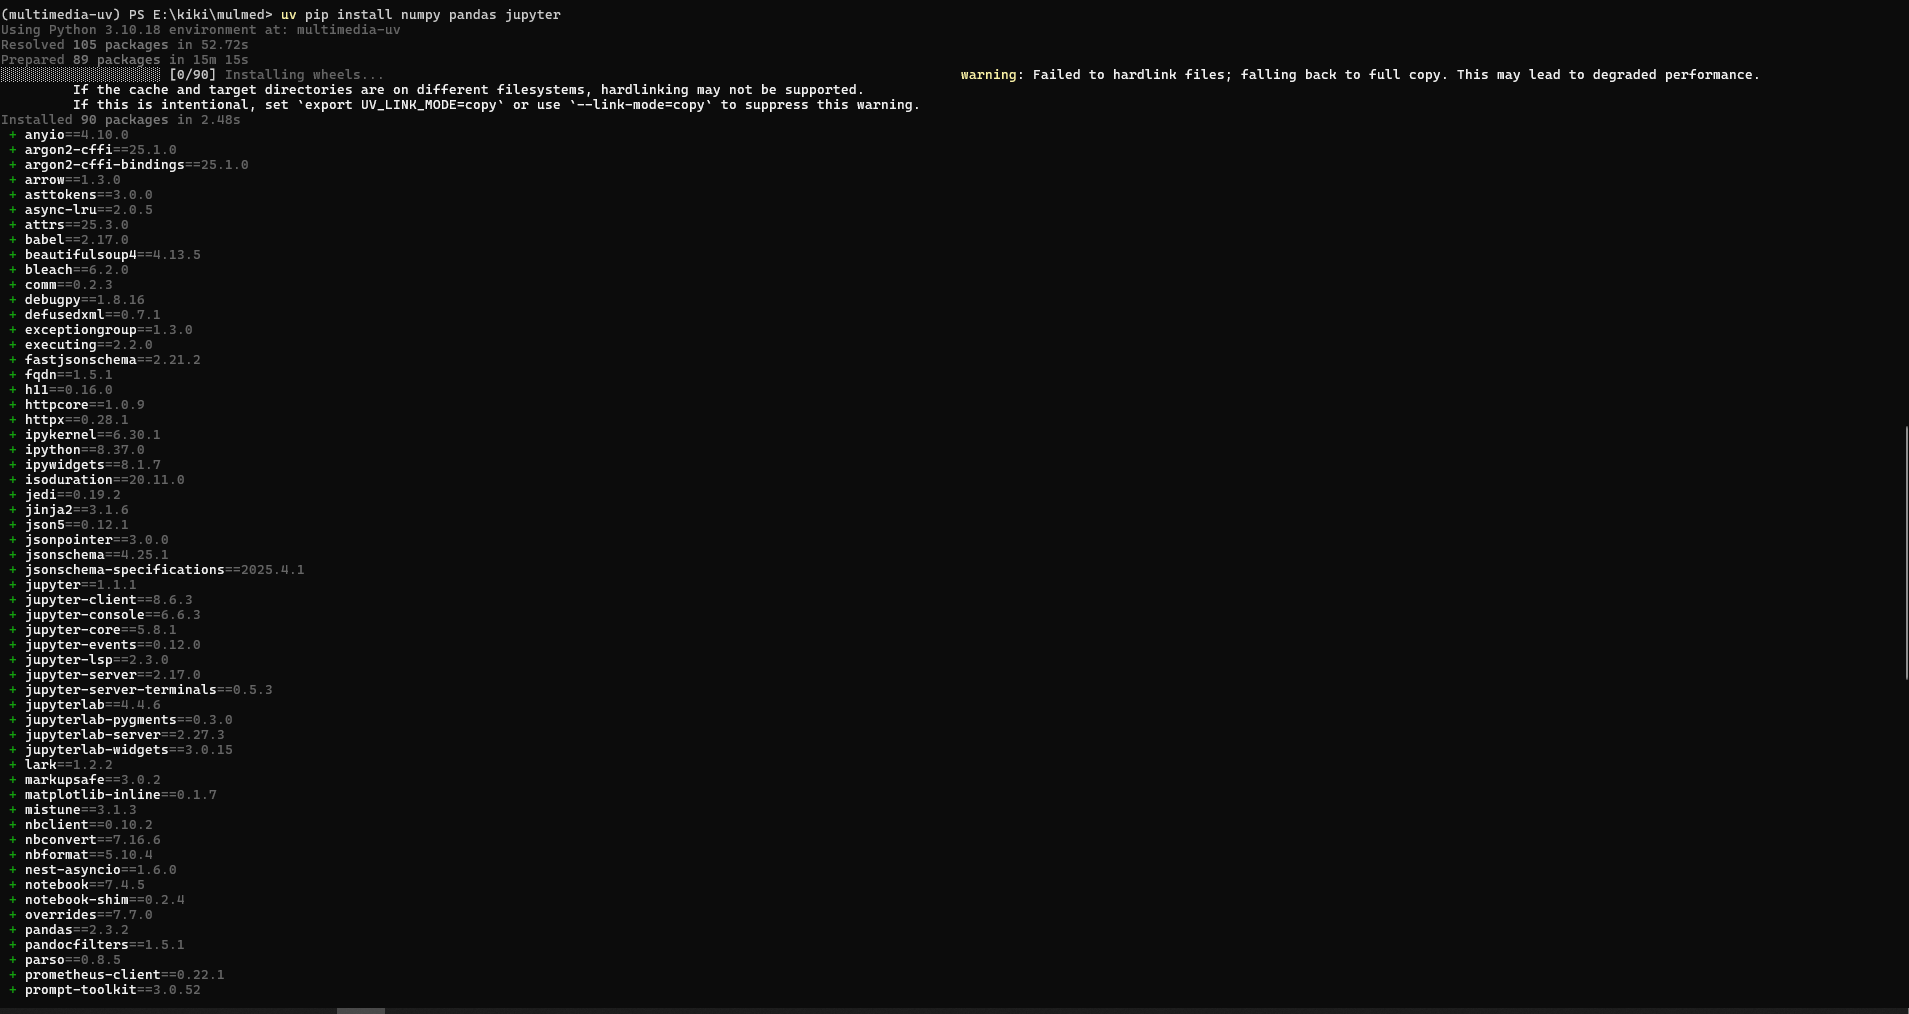
\includegraphics[width=\linewidth]{Figure/InstallGeneral.png}
                \caption{Instalasi library general purpose}
            \end{subfigure}

            \caption{Output instalasi library}
        \end{figure}

    \item Daftar library yang berhasil diinstall dengan versinya:
        \begin{multicols}{3}
        \raggedright
        \begin{Verbatim}[fontsize=\scriptsize]
anyio==4.10.0
argon2-cffi==25.1.0
argon2-cffi-bindings==25.1.0
arrow==1.3.0
asttokens==3.0.0
async-lru==2.0.5
attrs==25.3.0
audioread==3.0.1
babel==2.17.0
beautifulsoup4==4.13.5
bleach==6.2.0
certifi==2025.8.3
cffi==1.17.1
charset-normalizer==3.4.3
colorama==0.4.6
comm==0.2.3
contourpy==1.3.2
cycler==0.12.1
debugpy==1.8.16
decorator==5.2.1
defusedxml==0.7.1
exceptiongroup==1.3.0
executing==2.2.0
fastjsonschema==2.21.2
ffmpeg==1.4
fonttools==4.59.2
fqdn==1.5.1
h11==0.16.0
httpcore==1.0.9
httpx==0.28.1
idna==3.10
imageio==2.37.0
imageio-ffmpeg==0.6.0
ipykernel==6.30.1
ipython==8.37.0
ipywidgets==8.1.7
isoduration==20.11.0
jedi==0.19.2
jinja2==3.1.6
joblib==1.5.2
json5==0.12.1
jsonpointer==3.0.0
jsonschema==4.25.1
jsonschema-specifications==2025.4.1
jupyter==1.1.1
jupyter-client==8.6.3
jupyter-console==6.6.3
jupyter-core==5.8.1
jupyter-events==0.12.0
jupyter-lsp==2.3.0
jupyter-server==2.17.0
jupyter-server-terminals==0.5.3
jupyterlab==4.4.6
jupyterlab-pygments==0.3.0
jupyterlab-server==2.27.3
jupyterlab-widgets==3.0.15
kiwisolver==1.4.9
lark==1.2.2
lazy-loader==0.4
librosa==0.11.0
llvmlite==0.44.0
markupsafe==3.0.2
matplotlib==3.10.5
matplotlib-inline==0.1.7
mistune==3.1.3
moviepy==2.2.1
msgpack==1.1.1
nbclient==0.10.2
nbconvert==7.16.6
nbformat==5.10.4
nest-asyncio==1.6.0
networkx==3.4.2
notebook==7.4.5
notebook-shim==0.2.4
numba==0.61.2
numpy==2.2.6
opencv-python==4.12.0.88
overrides==7.7.0
packaging==25.0
pandas==2.3.2
pandocfilters==1.5.1
parso==0.8.5
pillow==11.3.0
platformdirs==4.4.0
pooch==1.8.2
proglog==0.1.12
prometheus-client==0.22.1
prompt-toolkit==3.0.52
psutil==7.0.0
pure-eval==0.2.3
pycparser==2.22
pygments==2.19.2
pyparsing==3.2.3
python-dateutil==2.9.0.post0
python-dotenv==1.1.1
python-json-logger==3.3.0
pytz==2025.2
pywin32==311
pywinpty==3.0.0
pyyaml==6.0.2
pyzmq==27.0.2
referencing==0.36.2
requests==2.32.5
rfc3339-validator==0.1.4
rfc3986-validator==0.1.1
rfc3987-syntax==1.1.0
rpds-py==0.27.1
scikit-image==0.25.2
scikit-learn==1.7.1
scipy==1.15.3
send2trash==1.8.3
setuptools==80.9.0
six==1.17.0
sniffio==1.3.1
soundfile==0.13.1
soupsieve==2.8
soxr==0.5.0.post1
stack-data==0.6.3
terminado==0.18.1
threadpoolctl==3.6.0
tifffile==2025.5.10
tinycss2==1.4.0
tomli==2.2.1
tornado==6.5.2
tqdm==4.67.1
traitlets==5.14.3
types-python-dateutil==2.9.0.20250822
typing-extensions==4.15.0
tzdata==2025.2
uri-template==1.3.0
urllib3==2.5.0
wcwidth==0.2.13
webcolors==24.11.1
webencodings==0.5.1
websocket-client==1.8.0
widgetsnbextension==4.0.14
        \end{Verbatim}
        \end{multicols}

\end{itemize}

\subsection{Bagian 3: Verifikasi Instalasi}
Buat file Python sederhana untuk menguji semua library yang telah diinstall:
\begin{lstlisting}[language=bash, caption=Kode pengujian library]
import pkg_resources

requirements = [
    "anyio==4.10.0",
    "argon2-cffi==25.1.0",
    "argon2-cffi-bindings==25.1.0",
    "arrow==1.3.0",
    "asttokens==3.0.0",
    "async-lru==2.0.5",
    "attrs==25.3.0",
    "audioread==3.0.1",
    "babel==2.17.0",
    "beautifulsoup4==4.13.5",
    "bleach==6.2.0",
    "certifi==2025.8.3",
    "cffi==1.17.1",
    "charset-normalizer==3.4.3",
    "colorama==0.4.6",
    "comm==0.2.3",
    "contourpy==1.3.2",
    "cycler==0.12.1",
    "debugpy==1.8.16",
    "decorator==5.2.1",
    "defusedxml==0.7.1",
    "exceptiongroup==1.3.0",
    "executing==2.2.0",
    "fastjsonschema==2.21.2",
    "ffmpeg==1.4",
    "fonttools==4.59.2",
    "fqdn==1.5.1",
    "h11==0.16.0",
    "httpcore==1.0.9",
    "httpx==0.28.1",
    "idna==3.10",
    "imageio==2.37.0",
    "imageio-ffmpeg==0.6.0",
    "ipykernel==6.30.1",
    "ipython==8.37.0",
    "ipywidgets==8.1.7",
    "isoduration==20.11.0",
    "jedi==0.19.2",
    "jinja2==3.1.6",
    "joblib==1.5.2",
    "json5==0.12.1",
    "jsonpointer==3.0.0",
    "jsonschema==4.25.1",
    "jsonschema-specifications==2025.4.1",
    "jupyter==1.1.1",
    "jupyter-client==8.6.3",
    "jupyter-console==6.6.3",
    "jupyter-core==5.8.1",
    "jupyter-events==0.12.0",
    "jupyter-lsp==2.3.0",
    "jupyter-server==2.17.0",
    "jupyter-server-terminals==0.5.3",
    "jupyterlab==4.4.6",
    "jupyterlab-pygments==0.3.0",
    "jupyterlab-server==2.27.3",
    "jupyterlab-widgets==3.0.15",
    "kiwisolver==1.4.9",
    "lark==1.2.2",
    "lazy-loader==0.4",
    "librosa==0.11.0",
    "llvmlite==0.44.0",
    "markupsafe==3.0.2",
    "matplotlib==3.10.5",
    "matplotlib-inline==0.1.7",
    "mistune==3.1.3",
    "moviepy==2.2.1",
    "msgpack==1.1.1",
    "nbclient==0.10.2",
    "nbconvert==7.16.6",
    "nbformat==5.10.4",
    "nest-asyncio==1.6.0",
    "networkx==3.4.2",
    "notebook==7.4.5",
    "notebook-shim==0.2.4",
    "numba==0.61.2",
    "numpy==2.2.6",
    "opencv-python==4.12.0.88",
    "overrides==7.7.0",
    "packaging==25.0",
    "pandas==2.3.2",
    "pandocfilters==1.5.1",
    "parso==0.8.5",
    "pillow==11.3.0",
    "platformdirs==4.4.0",
    "pooch==1.8.2",
    "proglog==0.1.12",
    "prometheus-client==0.22.1",
    "prompt-toolkit==3.0.52",
    "psutil==7.0.0",
    "pure-eval==0.2.3",
    "pycparser==2.22",
    "pygments==2.19.2",
    "pyparsing==3.2.3",
    "python-dateutil==2.9.0.post0",
    "python-dotenv==1.1.1",
    "python-json-logger==3.3.0",
    "pytz==2025.2",
    "pywin32==311",
    "pywinpty==3.0.0",
    "pyyaml==6.0.2",
    "pyzmq==27.0.2",
    "referencing==0.36.2",
    "requests==2.32.5",
    "rfc3339-validator==0.1.4",
    "rfc3986-validator==0.1.1",
    "rfc3987-syntax==1.1.0",
    "rpds-py==0.27.1",
    "scikit-image==0.25.2",
    "scikit-learn==1.7.1",
    "scipy==1.15.3",
    "send2trash==1.8.3",
    "setuptools==80.9.0",
    "six==1.17.0",
    "sniffio==1.3.1",
    "soundfile==0.13.1",
    "soupsieve==2.8",
    "soxr==0.5.0.post1",
    "stack-data==0.6.3",
    "terminado==0.18.1",
    "threadpoolctl==3.6.0",
    "tifffile==2025.5.10",
    "tinycss2==1.4.0",
    "tomli==2.2.1",
    "tornado==6.5.2",
    "tqdm==4.67.1",
    "traitlets==5.14.3",
    "types-python-dateutil==2.9.0.20250822",
    "typing-extensions==4.15.0",
    "tzdata==2025.2",
    "uri-template==1.3.0",
    "urllib3==2.5.0",
    "wcwidth==0.2.13",
    "webcolors==24.11.1",
    "webencodings==0.5.1",
    "websocket-client==1.8.0",
    "widgetsnbextension==4.0.14",
]

def check_requirements(reqs):
    installed_packages = {pkg.key: pkg.version for pkg in pkg_resources.working_set}

    print(f"{'Package':30} {'Required':15} {'Installed':15} Status")
    print("="*80)

    for req in reqs:
        try:
            req_pkg = pkg_resources.Requirement.parse(req)
            name = req_pkg.key
            required_version = str(req_pkg.specifier) if req_pkg.specifier else "Any"
        except Exception as e:
            print(f"{req:30} {'-':15} {'-':15} Error parsing")
            continue

        if name in installed_packages:
            installed_version = installed_packages[name]
            if req_pkg.specifier and installed_version not in req_pkg.specifier:
                status = "Version mismatch"
            else:
                status = "OK"
        else:
            installed_version = "-"
            status = "Missing"

        print(f"{name:30} {required_version:15} {installed_version:15} {status}")

if __name__ == "__main__":
    check_requirements(requirements)
\end{lstlisting}

\textbf{Jalankan script dan dokumentasikan hasilnya:}
    \begin{figure}[h!]
        \centering
        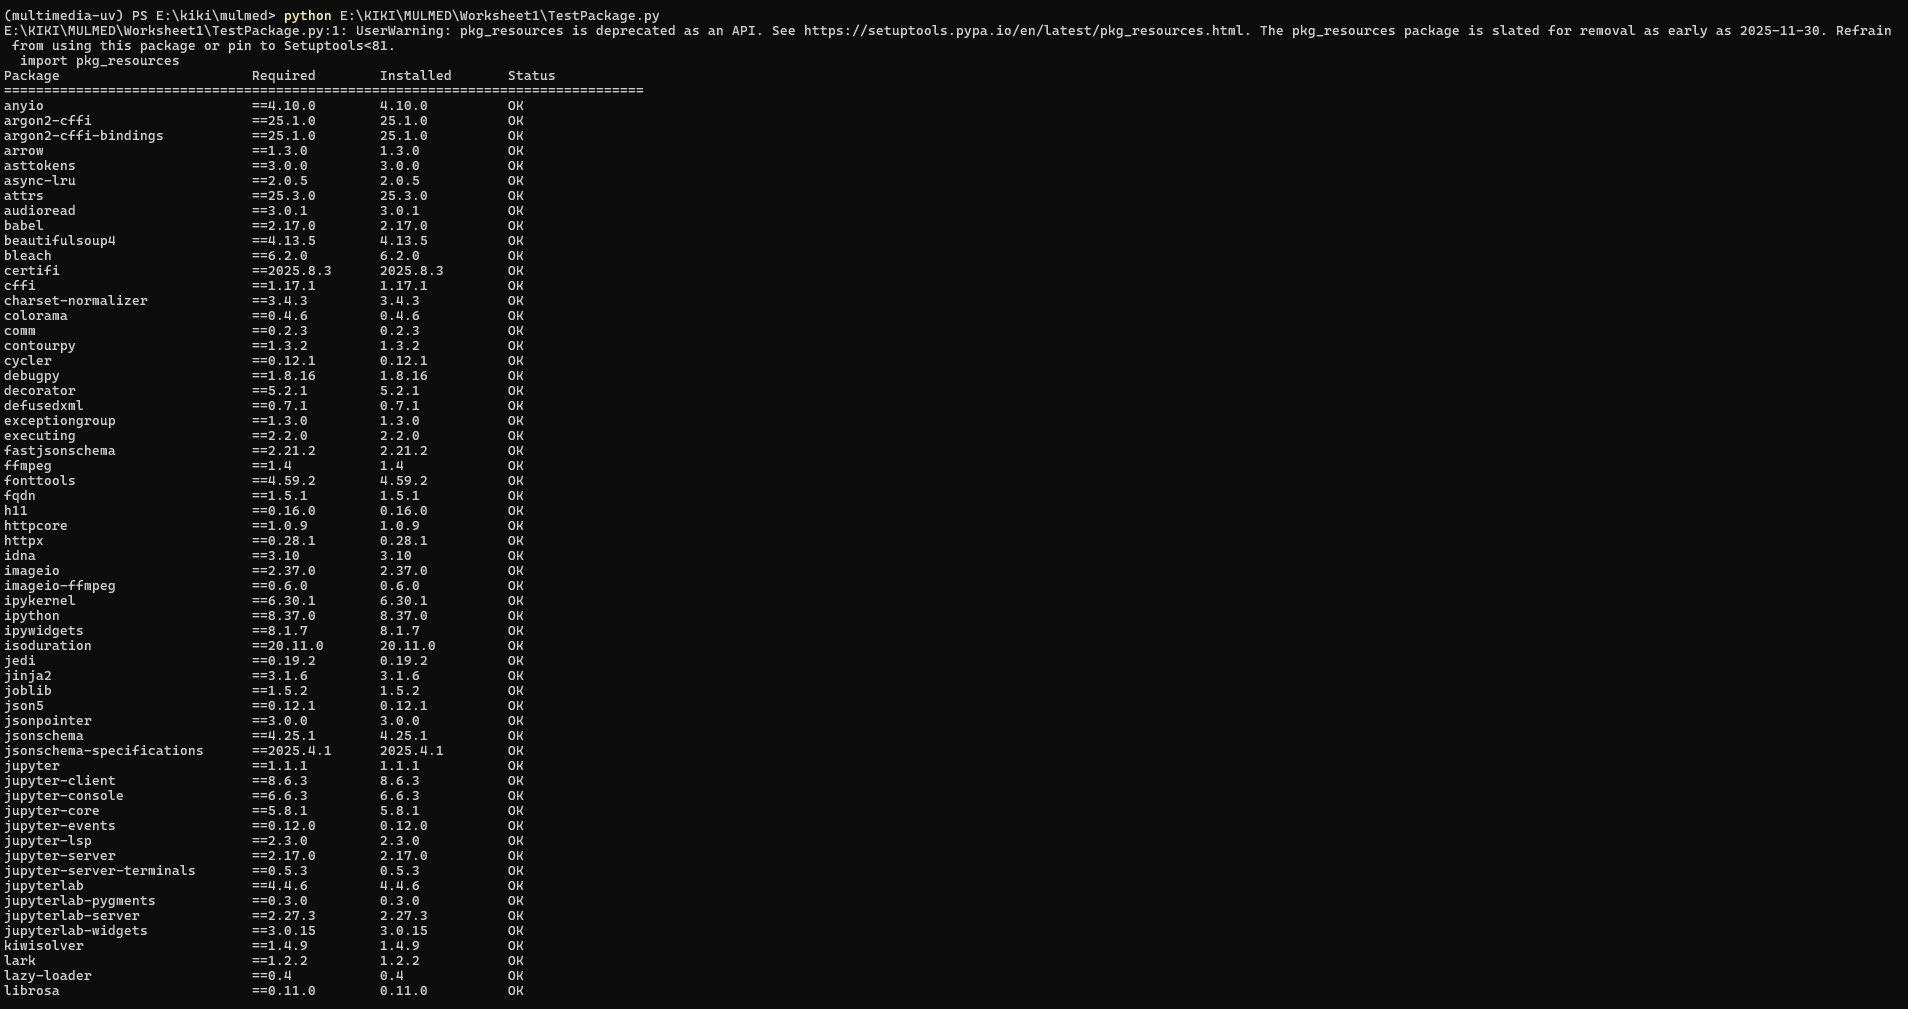
\includegraphics[scale = 0.33]{Figure/TestPackage.png}
        \caption{Output pengujian library} 
        \vspace{0.1cm}
    \end{figure}


\subsection{Bagian 4: Simple Test dengan Sample Code}
Buat dan jalankan contoh sederhana untuk setiap kategori multimedia:

\subsubsection{Test Audio Processing}
\begin{lstlisting}[language=Python, caption=Test audio processing sederhana]
import numpy as np
import matplotlib.pyplot as plt

# Generate simple sine wave
duration = 2  # seconds
sample_rate = 44100
frequency = 440  # A4 note

t = np.linspace(0, duration, int(sample_rate * duration))
audio_signal = np.sin(2 * np.pi * frequency * t)

# Plot waveform
plt.figure(figsize=(10, 4))
plt.plot(t[:1000], audio_signal[:1000])  # Plot first 1000 samples
plt.title('Sine Wave (440 Hz)')
plt.xlabel('Time (s)')
plt.ylabel('Amplitude')
plt.grid(True)
plt.savefig('sine_wave_test.png', dpi=150, bbox_inches='tight')
plt.show()

print(f"Generated {duration}s sine wave at {frequency}Hz")
print(f"Sample rate: {sample_rate}Hz")
print(f"Total samples: {len(audio_signal)}")
\end{lstlisting}

\subsubsection{Test Image Processing}
\begin{lstlisting}[language=Python, caption=Test image processing sederhana]
import numpy as np
import matplotlib.pyplot as plt
from PIL import Image

# Create a simple test image
width, height = 400, 300
image = np.zeros((height, width, 3), dtype=np.uint8)

# Add some patterns
image[:, :width//3, 0] = 255  # Red section
image[:, width//3:2*width//3, 1] = 255  # Green section
image[:, 2*width//3:, 2] = 255  # Blue section

# Add a white circle in the center
center_x, center_y = width//2, height//2
radius = 50
Y, X = np.ogrid[:height, :width]
mask = (X - center_x)**2 + (Y - center_y)**2 <= radius**2
image[mask] = [255, 255, 255]

# Display and save
plt.figure(figsize=(8, 6))
plt.imshow(image)
plt.title('Test Image with RGB Stripes and White Circle')
plt.axis('off')
plt.savefig('test_image.png', dpi=150, bbox_inches='tight')
plt.show()

print(f"Created test image: {width}x{height} pixels")
print(f"Image shape: {image.shape}")
print(f"Image dtype: {image.dtype}")
\end{lstlisting}

\textbf{Dokumentasikan hasil eksekusi:}
\begin{itemize}
    \item Screenshot output dari kedua script di atas
        \begin{figure}[h!]
        \centering
        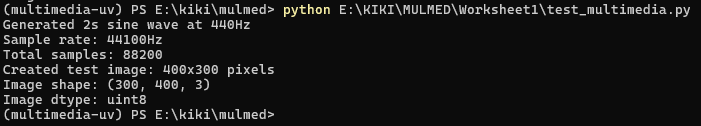
\includegraphics[scale = 0.84]{Figure/OutputMultimedia.png}
        \caption{Output pengujian library} 
        \vspace{0.1cm}
        \end{figure}
    \item Gambar yang dihasilkan (sine\_wave\_test.png dan test\_image.png)
        \begin{figure}[h]
            \centering
            \begin{subfigure}{0.48\textwidth}
                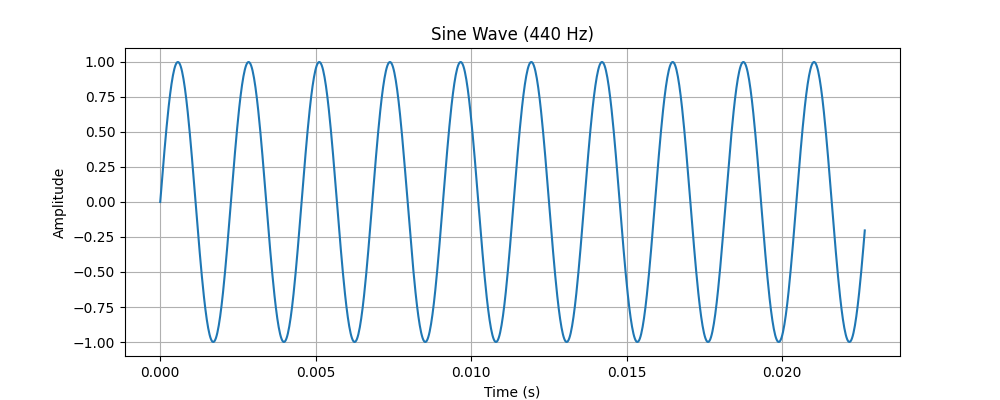
\includegraphics[width=\linewidth]{Figure/sine_wave_test.png}
                \caption{Visualisasi sine wave 440 Hz}
            \end{subfigure}
            \begin{subfigure}{0.48\textwidth}
                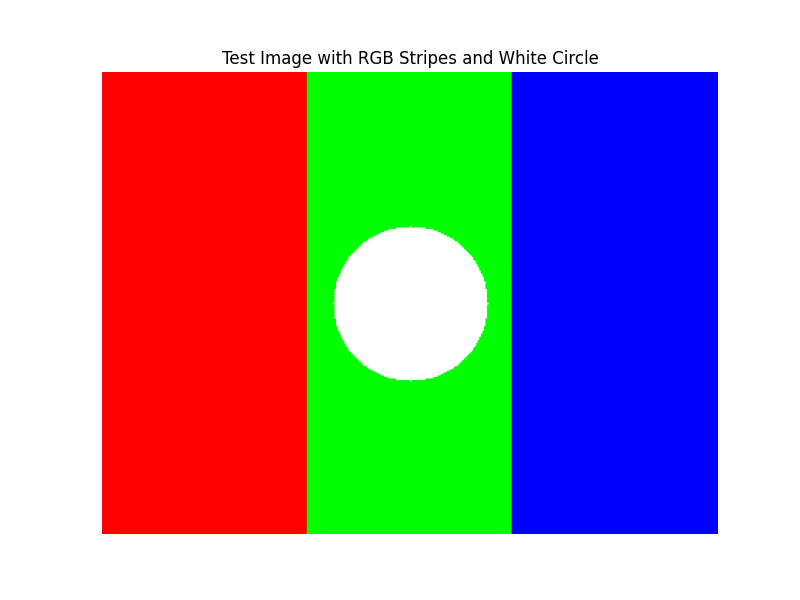
\includegraphics[width=\linewidth]{Figure/test_image.png}
                \caption{Visualisasi test image }
            \end{subfigure}
            \caption{Gambar yang dihasilkan dari script test multimedia}
        \end{figure}
\end{itemize}

\section{Bagian Laporan}

\subsection{Output Verifikasi Instalasi}
\textbf{Copy-paste output lengkap dari script \texttt{test\_multimedia.py} di sini:}

\begin{lstlisting}[caption=Output verifikasi instalasi]
Generated 2s sine wave at 440Hz
Sample rate: 44100Hz
Total samples: 88200
Created test image: 400x300 pixels
Image shape: (300, 400, 3)
Image dtype: uint8
\end{lstlisting}

\subsection{Screenshot Hasil Test}
\textbf{Sisipkan screenshot atau gambar hasil dari:}
\begin{itemize}
    \item Terminal/command prompt yang menunjukkan environment aktif
        \begin{figure}[H]
        \centering
        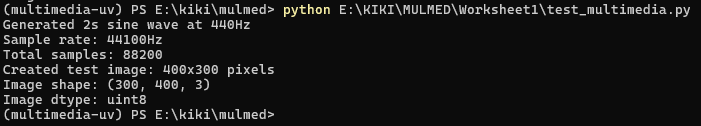
\includegraphics[scale=0.84]{Figure/OutputMultimedia.png}
        \caption{Output test multimedia di terminal} 
        \vspace{0.1cm}
        \end{figure}
    \item Output dari script test audio (sine wave plot)
        \begin{figure}[H]
        \centering
        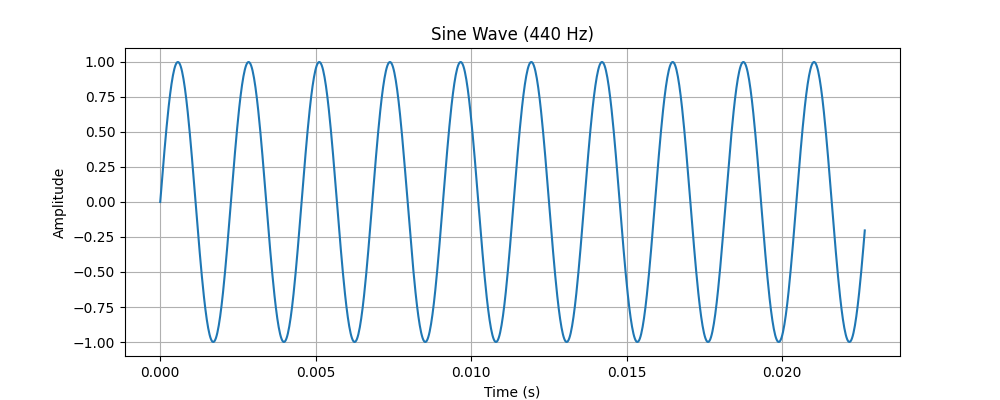
\includegraphics[scale=0.5]{Figure/sine_wave_test.png}
        \caption{Output test audio dengan sine wave 440 Hz} 
        \vspace{0.1cm}
        \end{figure}
    \item Output dari script test image (RGB stripes dengan circle)
        \begin{figure}[H]
        \centering
        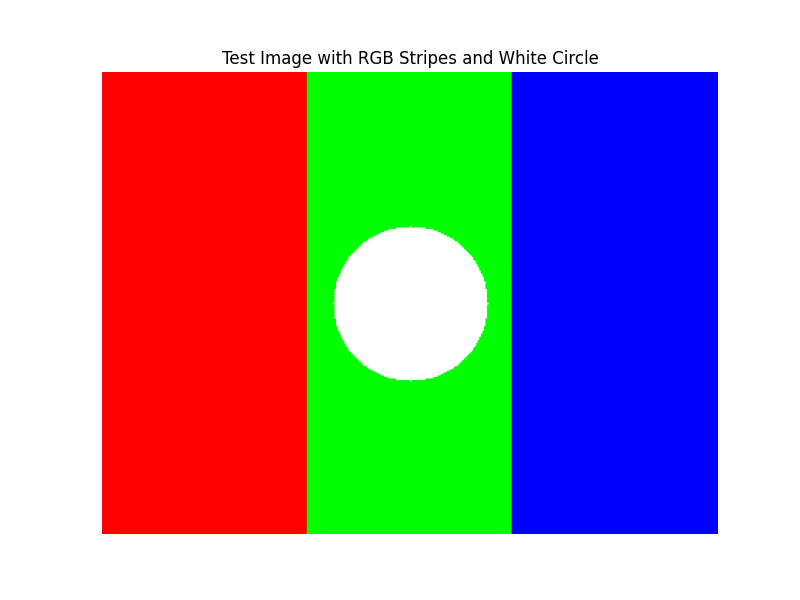
\includegraphics[scale=0.5]{Figure/test_image.png}
        \caption{Output test image dengan RGB stripes dan circle} 
        \vspace{0.1cm}
        \end{figure}
\end{itemize}

\subsection{Analisis dan Refleksi}
\textbf{Jawab pertanyaan berikut:}

\begin{enumerate}
    \item \textbf{Mengapa penting menggunakan environment terpisah untuk project multimedia?}
    
    \textit{Dengan mengungakan environment terpisah, kita dapat mengelola dependensi library yang spesifik untuk project multimedia tanpa mengganggu instalasi global Python atau project lain. Hal ini membantu mencegah konflik versi library dan memastikan bahwa project berjalan dengan konfigurasi yang konsisten.}
    
    \item \textbf{Apa perbedaan utama antara conda, venv, dan uv? Mengapa Anda memilih tool yang Anda gunakan?}
    
    \textit{Conda adalah manajer environment yang juga mengelola paket dan dependensi, sesuai mengelola dependensi kompleks di berbagai bahasa pemrograman. Venv adalah tool bawaan Python yang sederhana untuk membuat environment terisolasi dan sesuai untuk proyek-proyek sederhana yang hanya menggunakan Python, sedangkan uv adalah tool modern yang cepat dan mudah dan dirancang untuk mengelola lingkungan dan menginstal paket dengan efisiensi tinggi. Alasan memilih uv adalah karena kemudahan penggunaan dan kecepatan dalam membuat environment.}
    
    \item \textbf{Library mana yang paling sulit diinstall dan mengapa?}
    
    \textit{Sejauh ini, tidak ada library yang sulit diinstall. Semua library berhasil diinstall tanpa masalah.}
    
    \item \textbf{Bagaimana cara mengatasi masalah dependency conflict jika terjadi?}
    
    \textit{Untuk mengatasi masalah dependency conflict, saya mencoba beberapa langkah berikut:}
    \begin{itemize}
        \item \textit{Mencari tahu library mana yang menyebabkan konflik.}
        \item \textit{Menghapus library yang bermasalah dan menginstal ulang versi yang kompatibel.}
        \item \textit{Memeriksa dokumentasi resmi library untuk mengetahui versi yang kompatibel.}
        \item \textit{Menggunakan virtual environment terpisah untuk setiap project.}
        \item \textit{Mencari solusi di forum atau dokumentasi resmi library terkait.}
        \item \textit{Jika tetap tidak berhasil bertanya ke asisten virtual}
    \end{itemize}
    
    \item \textbf{Jelaskan fungsi dari masing-masing library yang berhasil Anda install!}
    \begin{itemize}
        \item \textit{\textbf{Librosa} digunakan untuk memuat, menganalisis, dan mengekstrak audio (MFCC, Spektogram mel, Kroma).}
        \item \textit{\textbf{soundfile} digunakan untuk membaca dan menulis berbagai berkas audio seperti WAV, FLAC, dll.}
        \item \textit{\textbf{scipy} digunakan untuk melakukan komputasi ilmiah dan matematika, seperti optimasi, aljabar linear, interpolasi, pemrosesan gambar dan sinyal, serta statistik.}
        \item \textit{\textbf{opencv-python} merupakan library yang diranang untuk melakukan pengeditan dan tugas-tugas computer vision.}
        \item \textit{\textbf{pillow} digunakan untuk memanipulasi gambar dan pemrosesan gambar dasar.}
        \item \textit{\textbf{scikit-image} adalah kumpulan algoritma yang digunakan untuk memproses gambar dan computer vision.}
        \item \textit{\textbf{matplotlib} digunakan untuk membuat visualisasi data secara menarik dan informatif}
        \item \textit{\textbf{moviepy} digunakan untuk mengedit dan memproses video.}
        \item \textit{\textbf{ffmpeg} merupakan kerangka kerja multimedia yang yang digunakan untuk menangani video, audio, dan berkas aliran multimedia lainnya.}
        \item \textit{\textbf{numpy} digunakan untuk melakukan perhitungan saintifik seperti matriks, aljabar, dan lainnya.}
        \item \textit{\textbf{pandas} digunakan untuk menganalisis, membersihkan, eksplorasi, dan manipulasi data }
        \item \textit{\textbf{jupyter} digunakan sebagai lingkungan interaktif yang memungkinkan pengguna untuk menulis dan menjalankan kode serta menyajikan hasilnya.}
    \end{itemize}
\end{enumerate}

\subsection{Troubleshooting}
\textbf{Dokumentasikan masalah yang Anda hadapi (jika ada) dan cara mengatasinya:}

\begin{itemize}
    \item \textbf{Masalah 1:} \textit{Permasalahan instalasi MikTex dan Strawberry Perl di Windows, karena terbalik dalam proses instalasi.}
    
    \textbf{Solusi:} \textit{menginstal ulang MikTex dan Strawberry Perl dengan urutan yang benar, yaitu menginstal Strawberry Perl terlebih dahulu, kemudian MikTex.}

    \item \textbf{Masalah 2:} \textit{Permasalahan dalam interpreter versi Python di VSCode yang tidak sesuai dengan versi environment yang dibuat.}
    
    \textbf{Solusi:} \textit{Bertanya ke teman (Fathan) untuk mengatasi masalah tersebut, kemudian mengubah interpreter di VSCode ke versi Python yang sesuai dengan environment yang telah dibuat.}
\end{itemize}

\section{Export Environment untuk Reproduksi}
Sebagai langkah terakhir, export environment Anda agar dapat direproduksi:

\subsection{Untuk venv/uv}
\begin{lstlisting}[language=bash, caption=Export pip requirements]
pip freeze > requirements.txt
\end{lstlisting}

\textbf{Copy-paste isi file environment.yml atau requirements.txt di sini:}

\begin{lstlisting}[caption=Environment/Requirements file]
anyio==4.10.0
argon2-cffi==25.1.0
argon2-cffi-bindings==25.1.0
arrow==1.3.0
asttokens==3.0.0
async-lru==2.0.5
attrs==25.3.0
audioread==3.0.1
babel==2.17.0
beautifulsoup4==4.13.5
bleach==6.2.0
certifi==2025.8.3
cffi==1.17.1
charset-normalizer==3.4.3
colorama==0.4.6
comm==0.2.3
contourpy==1.3.2
cycler==0.12.1
debugpy==1.8.16
decorator==5.2.1
defusedxml==0.7.1
exceptiongroup==1.3.0
executing==2.2.0
fastjsonschema==2.21.2
ffmpeg==1.4
fonttools==4.59.2
fqdn==1.5.1
h11==0.16.0
httpcore==1.0.9
httpx==0.28.1
idna==3.10
imageio==2.37.0
imageio-ffmpeg==0.6.0
ipykernel==6.30.1
ipython==8.37.0
ipywidgets==8.1.7
isoduration==20.11.0
jedi==0.19.2
jinja2==3.1.6
joblib==1.5.2
json5==0.12.1
jsonpointer==3.0.0
jsonschema==4.25.1
jsonschema-specifications==2025.4.1
jupyter==1.1.1
jupyter-client==8.6.3
jupyter-console==6.6.3
jupyter-core==5.8.1
jupyter-events==0.12.0
jupyter-lsp==2.3.0
jupyter-server==2.17.0
jupyter-server-terminals==0.5.3
jupyterlab==4.4.6
jupyterlab-pygments==0.3.0
jupyterlab-server==2.27.3
jupyterlab-widgets==3.0.15
kiwisolver==1.4.9
lark==1.2.2
lazy-loader==0.4
librosa==0.11.0
llvmlite==0.44.0
markupsafe==3.0.2
matplotlib==3.10.5
matplotlib-inline==0.1.7
mistune==3.1.3
moviepy==2.2.1
msgpack==1.1.1
nbclient==0.10.2
nbconvert==7.16.6
nbformat==5.10.4
nest-asyncio==1.6.0
networkx==3.4.2
notebook==7.4.5
notebook-shim==0.2.4
numba==0.61.2
numpy==2.2.6
opencv-python==4.12.0.88
overrides==7.7.0
packaging==25.0
pandas==2.3.2
pandocfilters==1.5.1
parso==0.8.5
pillow==11.3.0
platformdirs==4.4.0
pooch==1.8.2
proglog==0.1.12
prometheus-client==0.22.1
prompt-toolkit==3.0.52
psutil==7.0.0
pure-eval==0.2.3
pycparser==2.22
pygments==2.19.2
pyparsing==3.2.3
python-dateutil==2.9.0.post0
python-dotenv==1.1.1
python-json-logger==3.3.0
pytz==2025.2
pywin32==311
pywinpty==3.0.0
pyyaml==6.0.2
pyzmq==27.0.2
referencing==0.36.2
requests==2.32.5
rfc3339-validator==0.1.4
rfc3986-validator==0.1.1
rfc3987-syntax==1.1.0
rpds-py==0.27.1
scikit-image==0.25.2
scikit-learn==1.7.1
scipy==1.15.3
send2trash==1.8.3
setuptools==80.9.0
six==1.17.0
sniffio==1.3.1
soundfile==0.13.1
soupsieve==2.8
soxr==0.5.0.post1
stack-data==0.6.3
terminado==0.18.1
threadpoolctl==3.6.0
tifffile==2025.5.10
tinycss2==1.4.0
tomli==2.2.1
tornado==6.5.2
tqdm==4.67.1
traitlets==5.14.3
types-python-dateutil==2.9.0.20250822
typing-extensions==4.15.0
tzdata==2025.2
uri-template==1.3.0
urllib3==2.5.0
wcwidth==0.2.13
webcolors==24.11.1
webencodings==0.5.1
websocket-client==1.8.0
widgetsnbextension==4.0.14
\end{lstlisting}

\section{Kesimpulan}
\textbf{Tuliskan kesimpulan Anda mengenai:}
\begin{itemize}
    \item Pengalaman setup Python environment untuk multimedia
    \item Persiapan untuk project multimedia selanjutnya
    \item Saran untuk mahasiswa lain yang akan melakukan setup serupa
\end{itemize}

\textit{
Pemisahan dependensi environment perlu dilakukan untuk menghindari konflik antar library serta memastikan stabilitas sistem yang digunakan. Dengan cara ini, setiap proyek dapat berjalan pada lingkungannya masing-masing tanpa saling memengaruhi, sehingga kesalahan akibat perbedaan versi library dapat diminimalisasi. Selain itu, pemisahan environment juga membantu dalam mengoptimalkan penggunaan sumber daya, karena hanya library yang benar-benar dibutuhkan saja yang diinstal. Persiapan ke depannya adalah selalu membuat environment baru untuk setiap proyek yang berbeda, kemudian menyesuaikan instalasi library sesuai kebutuhan. Hal ini tidak hanya memudahkan dalam proses pengembangan, tetapi juga mempermudah proses debugging ketika terjadi kesalahan. Saran untuk mahasiswa yang melakukan hal serupa adalah membiasakan diri untuk memisahkan dependensi environment, menggunakan manajer environment yang sesuai, serta selalu membaca dokumentasi resmi agar memahami setiap alur dalam proses instalasi. Dengan demikian, pengelolaan environment akan menjadi lebih terstruktur, efisien, dan mendukung keberhasilan proyek.}


\section{Referensi}
\begin{itemize}
    \item \href{https://docs.astral.sh/uv/}{Astral UV Documentation}
    \item \href{https://chatgpt.com/share/68b08d34-bc40-8000-97fd-3ddee3ee6b4c}{ChatGPT}
\end{itemize}

\section{Lampiran}
\begin{itemize}
    \item \href{https://github.com/Alfariz11/Sistem-Teknologi-Multimedia}{GitHub}
\end{itemize}
\end{document}